\apendice{Planificación}

\section{Introducción}



\section{Planificación temporal}

Antes de empezar a practicar la metodología basada en sprints, hubo aproximadamente un mes de planificación de las mecánicas del juego. A pesar de que fuesen evolucionando a lo largo del proyecto, era indispensable tener claro dónde quería llegar.

Se utlizó una metodoligía basada en srpints similar a \emph{Scrum}, aunque no se ha seguido estrictamente ya que la reuniones eran semanales, no diarias. Para hacer ayudar al seguimiento se utilizó \emph{ZenHub}, un addon para Github que nos permite:
\begin{itemize}
    \item Establecer Milestones, a modo de Sprints
    \item Estimar el tiempo de las tareas en \emph{storypoints} que, en mi caso, equivalían a horas.
    \item monitorizar el prograso en forma de Burndowns
\end{itemize}

Debo apuntar que no se utilizó \emph{ZenHub}  desde el principio, por lo que los primeros sprint no se monitorizaron.


A continuación se muestra la evolución del proyecto a través de los Sprints.

\subsection{Sprint 0: [02/01 al 02/02] }
Tareas:
\begin{itemize}
    \item Crear la mecánica del juego mínima
\end{itemize}


En esta iteración se establece como objetivo tener ya un juego funcionando. Sólo es necesario que te deje jugar y cuente la puntuación.

\subsection{Sprint 1: [02/02 al 16/02]}

\begin{itemize}
     \item Estudiar la posibilidad de poner el juego en una web. 
     \item Barajar diferentes formas de capturar los estados del juego. \item Valorar formas de comunicar el juego con las bibliotecas de \enoh{Python}.
\end{itemize}

En primer lugar, se han estado analizando qué posibilidades habría de alojar el juego en una web, ya que vamos a necesitar que muchos usuarios jueguen. \emph{Unity} te permite compilar directamente en \emph{WebGL} lo que me facilita mucho la tarea. Los problemas llegan cuando intento salvar datos del lado del servidor, no hubo manera de conseguir que el jugo guardase un solo archivo. Por este motivo se descartó la posibilidad de \emph{hostearlo} en un servidor web.

En este sprint también comienzo el proceso de definición de lo que conformarán las instancias. En las primeras pruebas tuve problemas al capturar las instancias, pues no había contemplado que el tamaño de estas fuese constante, requisito indispensable para el tipo de algoritmos de aprendizaje que estaba utilizando.

Para este sprint era interesante ir teniendo un primer contacto con las bibliotecas de \emph{sckit-learn}.

Como el juego ya estabe en funcionamiento comienzo a desarrollar is propios sprites para el juego.


\subsection{Sprint 2: [16/02 al 02/03]}

 En esta reunión se solucionó el problema de que TextMaker estaba mal instalado.
\begin{itemize}
    \item Se ha observado que la estimación de la isues no se estaba realizando correctamente.
    Se han comentado los siguientes temas: Para este proyecto va a ser necesario comunicar python y C\# por lo que se deberá investigar la forma de hacerlo.
\end{itemize}

En este punto es cuando realmente empiezo una dinámica similar a \emph{Scrumm}, en la que se harán reuniones, a ser posible, semanales, ya que antes estaba trabajando sin tener un objetivo semanal concreto.

El grueso del trabajo y el tiempo de este sprint lo absorbe la «odisea» que fue, para mi, el proceso de comunicar los scripts de \emph{Python} y Unity. Todo este proceso viene descrito en la memoria.

En el anterior sprint se observa que el jugador puede quedarse disparando continuamente, lo que quitaría emoción al juego. Por este motivo se propone que se implemente un sistema de «calentamiento» del arma, de este modo, el jugador se verá forzado a dejar de disparar. Junto con el calentamiento del arma viene, forzosamente, diseñar algún elemento gráfico que indique al jugador el estado del arma.

Llegados a este punto, se comienza a diseñar el menú de inicio.


\subsection{Sprint 3:  [02/03 al 14/03]}


En este sprint se validaron los avances hechos. La nueva interfaz estaba lista, la barra de calentamiento del arma funcionaba y el arma funcionaba como se espraba.

Respecto a la comunicación:
La opción mas viable hasta la fecha para la comunicación entre aplicaciones es la utilización de Pipes. De momento no tengo muy claro como funcionan. Los pipes en python utilizan un método (os.fork) que es específico de Linux. Me planteo descartar el uso de pipes y probar con sockets.


\subsection{Sprint 4:  [14/03 al 19/03]}

Se ha conseguido hacer funcionar sockets en \emph{Python}. Ahora hay que establecer la comunicación entre python y .net. Una vez conseguido esto se harán las primeras pruebas con el bot.

Para este sprint se pretende:
\begin{itemize}
    \item Una vez se ha hecho funcionar los sockets entre dos scripts de \emph{Python} se tiene que hacer entre una Unity y \emph{Python}.
    \item Si se consigue establecer la comunicación empezar a procesar estados.
    \item Entrenar un agente inteligente sencillo y probar si funciona la comunicación.
\end{itemize}



\subsection{Sprint 5: [21/03 al 28/03]}

Durante el sprint 4 encontré algunas dificultades. Había un error, de procedencia desconocida, que hacía que el juego parase la ejecución al pulsar la barra espaciadora. Este problema se solucionó refactorizando el código de controlador del jugador. Se consiguió comunicar Unity con \emph{Python} y ya tenía funcionando un bot simple.

Tarea para este Sprint: 
\begin{itemize}
    \item Respecto al estado:
    \begin{itemize}
        \item Añadir TimeStamp, vida restante de los enemigos y temperatura del arma.
        \item Ahora los estado pasarán a tener dos clases (Dirección del movimiento y si dispara o no).
    \end{itemize}
    \item Permitir moverse adelante y atrás.
    \item Dejar el juego funcional para poder pasar a la toma de datos.
    \item Añadir Banda sonora.
\end{itemize}


\subsection{Sprint 6: [28/03 al 12/04]}

En esta reunión se mostró la nueva interfaz y el juego listo para el entrenamiento. Para este sprint se pretende tener una IA básica funcionando con el nuevo set de estados y si todo va bien distribuir el juego entre otras personas para la captura de datos.

Respecto a las mejoras del juego:
\begin{itemize}
    \item El juego ya dispone de banda sonora. He intentado dar crédito a su autor, pero no he sido capaz de encontrarlo de nuevo (fallo mío no guardar el enlace).
    \item Se han incluido efectos de sonido para disparo, explosión y disparo.
    \item Ahora se almacenan las máximas puntuaciones a título meramente informativo.
    \item Los enemigos muestran, ahora, su barra de vida restante.
    \item Se incorporan dos tipos de «power-up»:
    \begin{itemize}
        \item Enfriar el arma: reduce una determinada la temperatura actual del arma.
        \item Boost: Duplica el arma, disparando el doble de balas en el mismo tiempo.
    \end{itemize}
    \item Permite moverse al jugador adelante y atrás.
    \item Nueva forma de perder, si el jugador impacta contra un enemigo, muere.
    \item Se incorpora un fundido a negro cuando se pasa del menú al juego.
\end{itemize}



\subsection{Sprint 7:  [12/04 al 18/04]}

Se ha observado que el método que captura los estado busca los enemigos aleatoriamente, de forma que si hace una lista con los enemigos de 1 al 6. El que es el enemigo $1$ en un primer instante puede ser almacenado como enemigo $3$ en otro. Se requiere un pre-procesado de los enemigos de tal forma que solo se tendrá en cuenta el número de enemigos hay en el eje $X$ y la distancia que han recorrido. Este es el punto en el que se incorpora el «heat-map» que de detalla en la memoria.

En este sprint se pretende tener el Bot entrenado con el nuevo conjunto de datos. Como hemos introducido una forma de diferente de procesar los enemigos, hay que adaptar los scripts a las nuevas instancias.

\begin{figure}[h!]
    \centering
    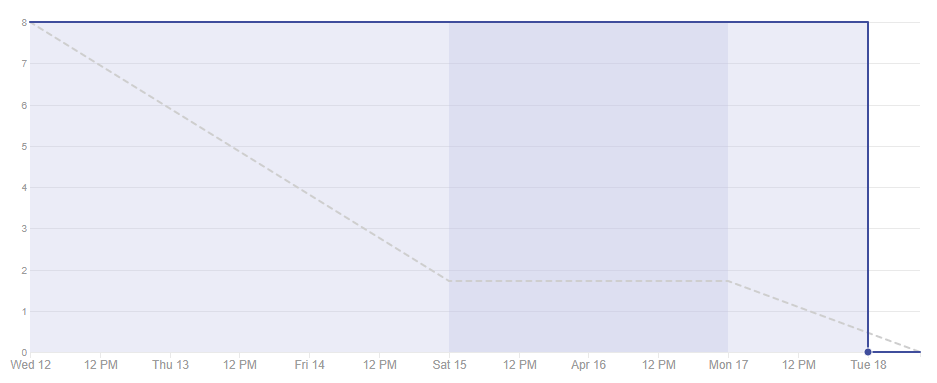
\includegraphics[width=\textwidth]{sprint7}
    \caption{Sprint 7}
    \label{fig:s7}
\end{figure}



\subsection{Sprint 8: [18/04 al 25/04]}

Se tiene que hacer un preprocesado del estado del juego a la hora de pasárselo al bot entrenado. (Me entran dudas de si seguiré siendo capaz de procesar 4 estados por segundo). Finalmente si que es posible, aunque en ocasiones pierde fotogramas. Esta pérdida la atribuyo a que mi ordenador es de gama baja.

El juego ya tiene la capacidad de jugar solo aunque sin demasiado acierto. Una vez completado el preprocesado se harán grupos de $n$ estados con el fin de tener en cuenta los $n$ estados anteriores a la toma de decisión, tal y como lo haría un humano. Esto se ha de hacer en python ya que a partir de ahora los estados generados por el juego es conveniente que sean invariables.

\begin{figure}[h!]
    \centering
    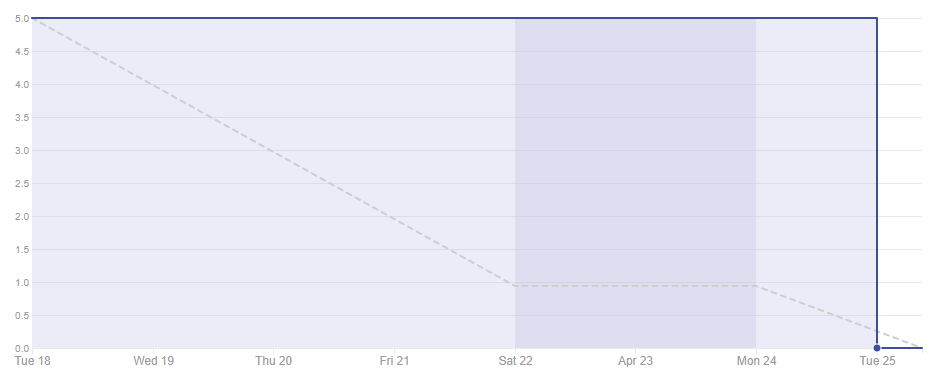
\includegraphics[width=\textwidth]{sprint8}
    \caption{Sprint 8}
    \label{fig:s8}
\end{figure}

\subsection{Sprint 9: [25/04 al 05/05]}

Se han barajado mejoras de aprendizaje supervisado: 
\begin{itemize}
    \item Parametrizar numero de estados anteriores
    \item Balancear clases: Esto significa que si, por ejemplo, estamos disparando el 90\% del tiempo, deberíamos eliminar las instancias necesarias para que las instancias queden proporcionalmente balanceadas 50\% disparando 50\% sin disparar. 
    \item Filtrar datos de buenos jugadores.
\end{itemize}
  
  A la vista de los resultados se opta por añadir un array que indique la proximidad a los enemigos. esto en teoría debería reforzar la tendencia a conductas suicidas
  

\begin{figure}[h!]
    \centering
    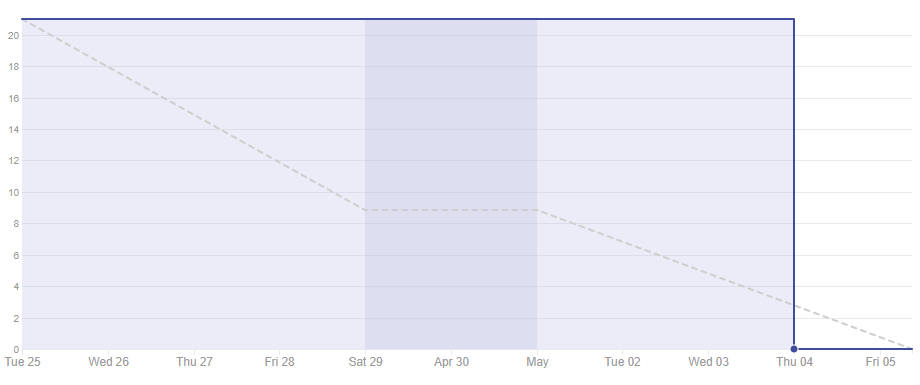
\includegraphics[width=\textwidth]{sprint9}
    \caption{Sprint 9}
    \label{fig:s9}
\end{figure}

\subsection{Sprint 10: [05/05 al 16/05]}

Ésta semana no ha habido grandes avances, se ha incorporado la detección de enemigos cercanos y se han analizado las posibles alternativas para seguir mejorando el aprendizaje.

Para este sprint se pretende refactorizar el código de los «power-up» : Fijar el código en una clase propia y no en el Player Controller.

\begin{figure}[h!]
    \centering
    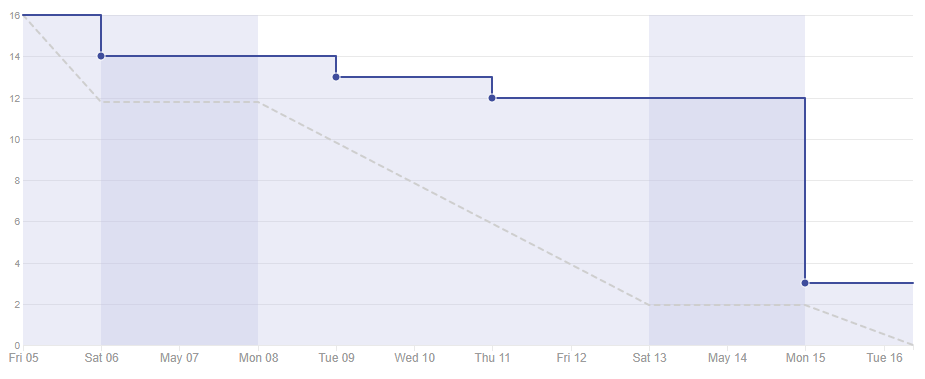
\includegraphics[width=\textwidth]{sprint10}
    \caption{Sprint 10}
    \label{fig:s10}
\end{figure}


\subsection{Sprint 11: [16/05 al 23/05]}

Se han aprobado los cambios. pasamos a la fase de entrenamiento con algoritmos evolutivos.
Propuestas:
\begin{itemize}
    \item Crear una pequeña aplicación unity que permita ser ejecutada desde línea de comando para ver si podemos lanzar el juego para el entrenamiento con algoritmos evolutivos.
    \item Rehacer las instancias para ver si podemos mejorar un poco más el entrenamiento por imitación.
    \item Hacer un script que nos haga de entrenador, generando el modelo del agente inteligente.
    \item Implementar un perceptrón sencillo para ver de qué soy capaz.
\end{itemize} 

\begin{figure}[h!]
    \centering
    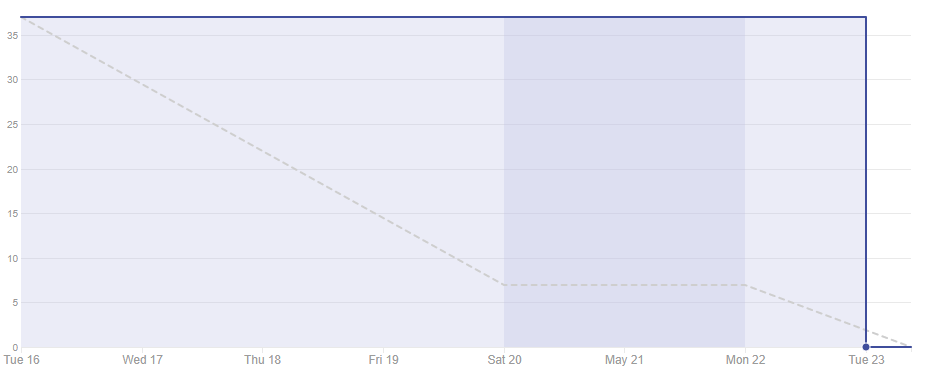
\includegraphics[width=\textwidth]{sprint11}
    \caption{Sprint 11}
    \label{fig:s11}
\end{figure}

\subsection{Sprint 12: [23/05 al 30/05]}

Se ha logrado utilizar un preceptrón multicapa para jugar al juego. Queda concatenar estado ya que juega bastante mal.

En este sprint se debe:
\begin{itemize}
    \item Jugar con los parámetros del percetrón para ver si mejora.
    \item Añadir información a las instancias: Actualmente solo ve a lo enemigos y su distancia relativa, hay que añadir la distancia relativa a paredes y power ups en la instancia. 
\end{itemize}

\begin{figure}[h!]
    \centering
    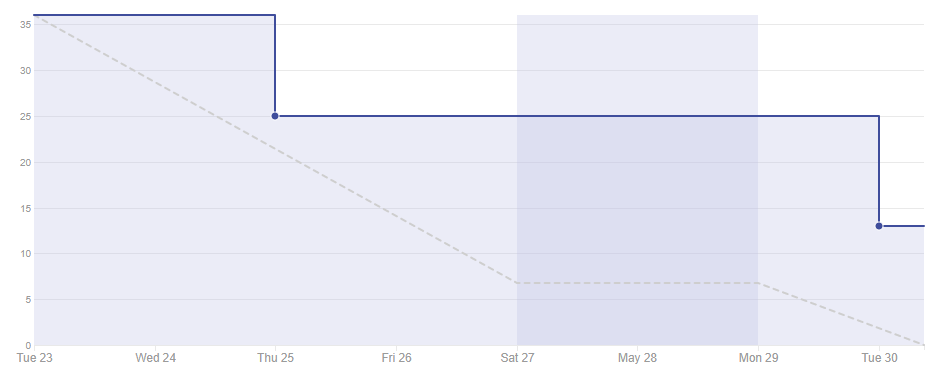
\includegraphics[width=\textwidth]{sprint12}
    \caption{Sprint 12}
    \label{fig:s12}
\end{figure}

\subsection{Sprint 13: [30/05 al 10/06]}

En este sprint se trabajará principalmente en la documentación. Hacer la explicación completa de los conceptos teóricos.


\subsection{Sprint 14:  10/06, 13/06}

Como en el sprint anterior no se pudo hacer el apartado Conceptos teóricos, queda pendiente para este. Si es posible se acabará el apartado Aspectos relevantes y se comenzará a trabajar con los anexos. Se han seguido haciendo pruebas con los algoritmos evolutivos.

\begin{figure}[h!]
    \centering
    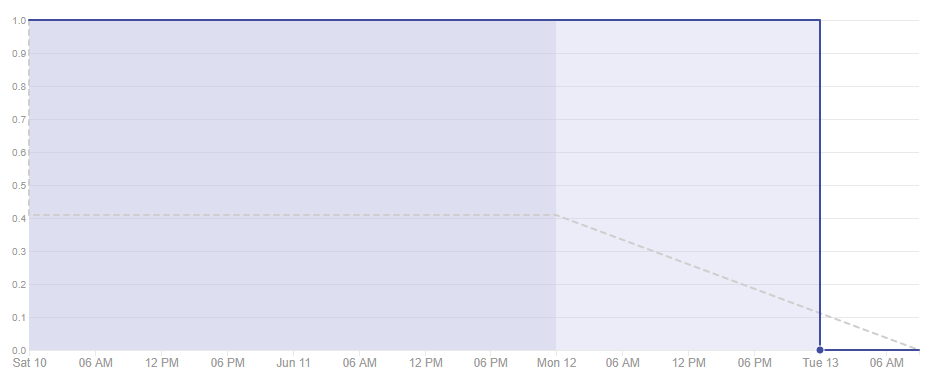
\includegraphics[width=\textwidth]{sprint14}
    \caption{Sprint 14}
    \label{fig:s14}
\end{figure}

\subsection{Sprint 15: [13/06 al 19/06]}

En este sprint se han realizado las siguientes tareas: 
\begin{itemize}
    \item Se ha corregido una series de errores que calificaría como graves, ya que impedían por completo la evolución de la red neuronal.
    \item Se han corregido errores tipográficos y conceptuales en la documentación. Había algunos aspectos que se entendieron mal inicialmente, se ha procedido a redactarlos de nuevo.
    \item Se ha seguido avanzando el los aspectos relevantes y los conceptos teóricos.
    \item Se ha generado una versión del juego para capturar los datos de los usuarios.
\end{itemize}

\subsection{Sprint 16: [19/06 al 28/06]}

Se pretende completar la documentación y corregir ciertos aspectos de los scripts.

\begin{figure}[h!]
    \centering
    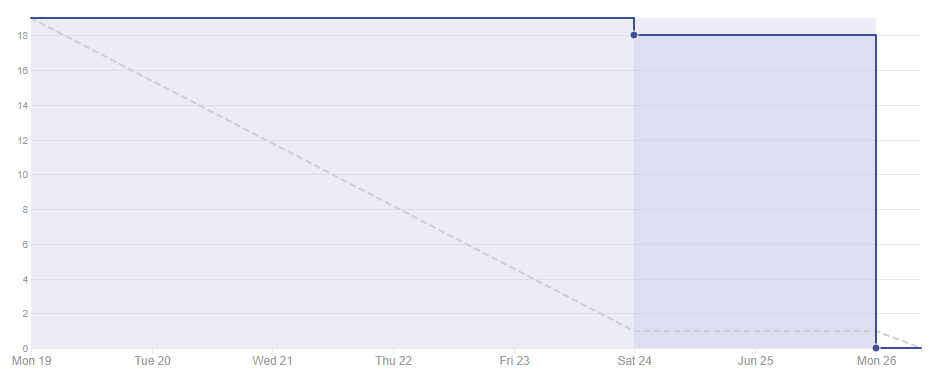
\includegraphics[width=\textwidth]{sprint16}
    \caption{Sprint 16}
    \label{fig:s16}
\end{figure}


\section{Estudio de viabilidad}

\subsection{Viabilidad económica}
Este proyecto nunca estuvo pensado para obtener un beneficio económico. Este proyecto tenía un objetivo claro, ampliar mis conocimientos en el campo de la inteligencia artificial y, de algún modo, dotar a futuros estudiantes de un entorno de trabajo mas vistoso sobre el que probar sus agentes inteligentes, y así, animar a los estudiante a descubrir el maravilloso mundo de la inteligencia artificial.

Analizando los costes, el único que nos podría limitar sería Unity3D, pero el acuerdo de licencia estipula que el uso de su software gratuito siempre que se utilice con fines educativos.

\subsection{Viabilidad legal}

Este proyecto ha sido realizado utilizando recursos de software, cada uno con su licencia. A continuación procedo a analizar cada uno de ellos:
\begin{itemize}
    \item Scikit-Learn: sujeto a la licencia de tipo BSD-3, que permite la redistribución con o sin modificaciones siempre que los autores originales sean mencionados y se mantenga el mismo tipo de licencia.
    \item Deap: se encuentra bajo licencia GNU GPL, que permite usar, copiar, modificar el software y redistribuirlo.
    \item Pandas: Pandas, al igual que scikit-learn, está sujeto a licencia BSD-3 y, por lo tanto, conlleva el mismo tipo de permisos y restricciones.
    \item Pickle: Esta biblioteca también se encuentra sujeta a los términos de BSD-3, por lo que ya hemos mencionado sus características. 
    \item Unity3D: Unity3D ofrece varios tipos de licencias \footnote{consultar detalles:  }
\end{itemize}


Debido a las restricciones de las licencias antes mencionadas mi proyecto, de ser distribuido, debería ser publicado bajo una licencia BSD \cite{wiki:BSD}.